\documentclass[10pt,twocolumn,letterpaper]{article}

\usepackage{acvs}
\usepackage{times}
\usepackage{epsfig}
\usepackage{graphicx}
\usepackage{amsmath}
\usepackage{amssymb}

% Include other packages here, before hyperref.

% If you comment hyperref and then uncomment it, you should delete
% egpaper.aux before re-running latex.  (Or just hit 'q' on the first latex
% run, let it finish, and you should be clear).
\usepackage[pagebackref=true,breaklinks=true,letterpaper=true,colorlinks,bookmarks=false]{hyperref}

\iccvfinalcopy % *** Uncomment this line for the final submission

\def\iccvPaperID{} % *** Enter the Paper ID here
\def\httilde{\mbox{\tt\raisebox{-.5ex}{\symbol{126}}}}

% Pages are numbered in submission mode, and unnumbered in camera-ready
\ificcvfinal\pagestyle{empty}\fi

\begin{document}

%%%%%%%%% TITLE - PLEASE UPDATE
\title{An Image is Worth 16 $\times$ 16 Words: Transformers for Image Recognition at Scale~\cite{vit} \\ {\rm {\normalsize Minji Kim (minji@snu.ac.kr; 2020-28702), Dept. of Electrical and Computer Engineering, Seoul National University}}}   % **** Enter the paper title and student information here

\maketitle
\thispagestyle{empty}

%%%%%%%%% BODY TEXT - ENTER YOUR RESPONSE BELOW

%%%%%%%%%%%%%%%%%
%%%%%%%%%%%%%%%%%
\section{Introduction}
While Transformer~\cite{transformer}-based architecture has become a popular choice in the field of natural language processing (NLP), convolutional architecture such as ResNet has remained dominant in computer vision.
Inspired by the success of the self-attention mechanism in NLP, lots of researches tried to combine the self-attention operation into CNN-like architectures, but none of them were entirely free of convolutions.
This work is the first approach to replace the most part of the convolutional operations (except for the early layer) into self-attention and multi-layer perceptron (MLP) layers to generalize the Transformer architecture in the image domain.
To do so, they split an image into patches and provide the sequence of linear embeddings of these patches as an input to a Transformer, while image patches are treated the same as tokens (words) in an NLP application.
The experimental results show that the pre-trained Vision Transformer (ViT) is effective for downstream tasks such as image recognition.


%%%%%%%%%%%%%%%%%
%%%%%%%%%%%%%%%%%
\section{Vision Transformer (ViT)}
\paragraph{Overview.}
An overview of the model is summarized in Fig.~\ref{fig:vit_overview}.
We split the input image $\mathbf{x} \in \mathbb{R}^{H \times W \times C}$ into fixed-size patches and flatten them into 2D as a form of $\mathbf{x}_p \in \mathbb{R}^{N \times (P^2 \cdot C)}$, where $(P,P)$ is the resolution of each image patch and $N=HW/P^2$ is the resulting number of patches.
The flattened patches are linearly projected to $D$ dimensions.
Similar to BERT's \texttt{[class]} token, a learnable embedding is added to the sequence of embedded patches ($\mathbf{z}^0_0 = \mathbf{x}_{\mathrm{class}}$), whose state at the output of the Transformer encoder ($\mathbf{z}^0_L$) becomes the image representation $\mathbf{y}$ after a layernorm operation (LN).
Before the Transformer encoder, learnable 1D positional embeddings are attached to the patch embeddings to retain positional information.
The Transformer encoder consists of multi-headed self attention (MSA), MLP blocks, where the MLP contains two layers with a GELU non-linearity and the LN and residual connections are applied before and after every block, respectively.

\paragraph{Inductive bias.}
While the self-attention layers of ViT are robust to capture the global relationship, they has much less image-specific inductive bias than CNNs where locality, two-dimensional neighborhood structure, and translation equivariance are included in each layer throughout the whole model.
This lack of inductive bias is helpful for the robustness and generalization ability but makes the convergence to be challenging and requires much large data for the performance improvement.

\paragraph{Fine-tuning.}
ViT is pre-trained on large datasets and fine-tuned on downstream tasks.
The model is typically fine-tuned with higher input resolutions since it is often beneficial for the performance improvement.
The patch size is remained same while the sequence length is increased; the pre-trained positional embeddings are linearly interpolated to fit in the location in the new image.



%%%%%%%%%%%%%%%%%
%%%%%%%%%%%%%%%%%
\section{Analysis}
\paragraph{Dataset size.}
ViT models show better performance on downstream tasks when they are pre-trained with larger dataset.
When pre-trained on ImageNet scale, ViT models perform worse than ResNet models due to the lack of inductive bias.

\paragraph{Self-supervision.}
With the masked patch prediction for self-supervision (similar to the BERT's strategy), ViT model shows 2\%p improvement to training from scratch, but still 4\%p behind the supervised version.


\paragraph{Limitations.}
While ViT opens the promising way for large-scale pre-training Transformer architecture,
there exist realistic constraints for directly pre-training such models such as the lack of computational resources and datasets (\eg, JFT-300M dataset is not publicly released).
Future directions might include how to improve the efficiency in pre-training.




\begin{figure}[t]
    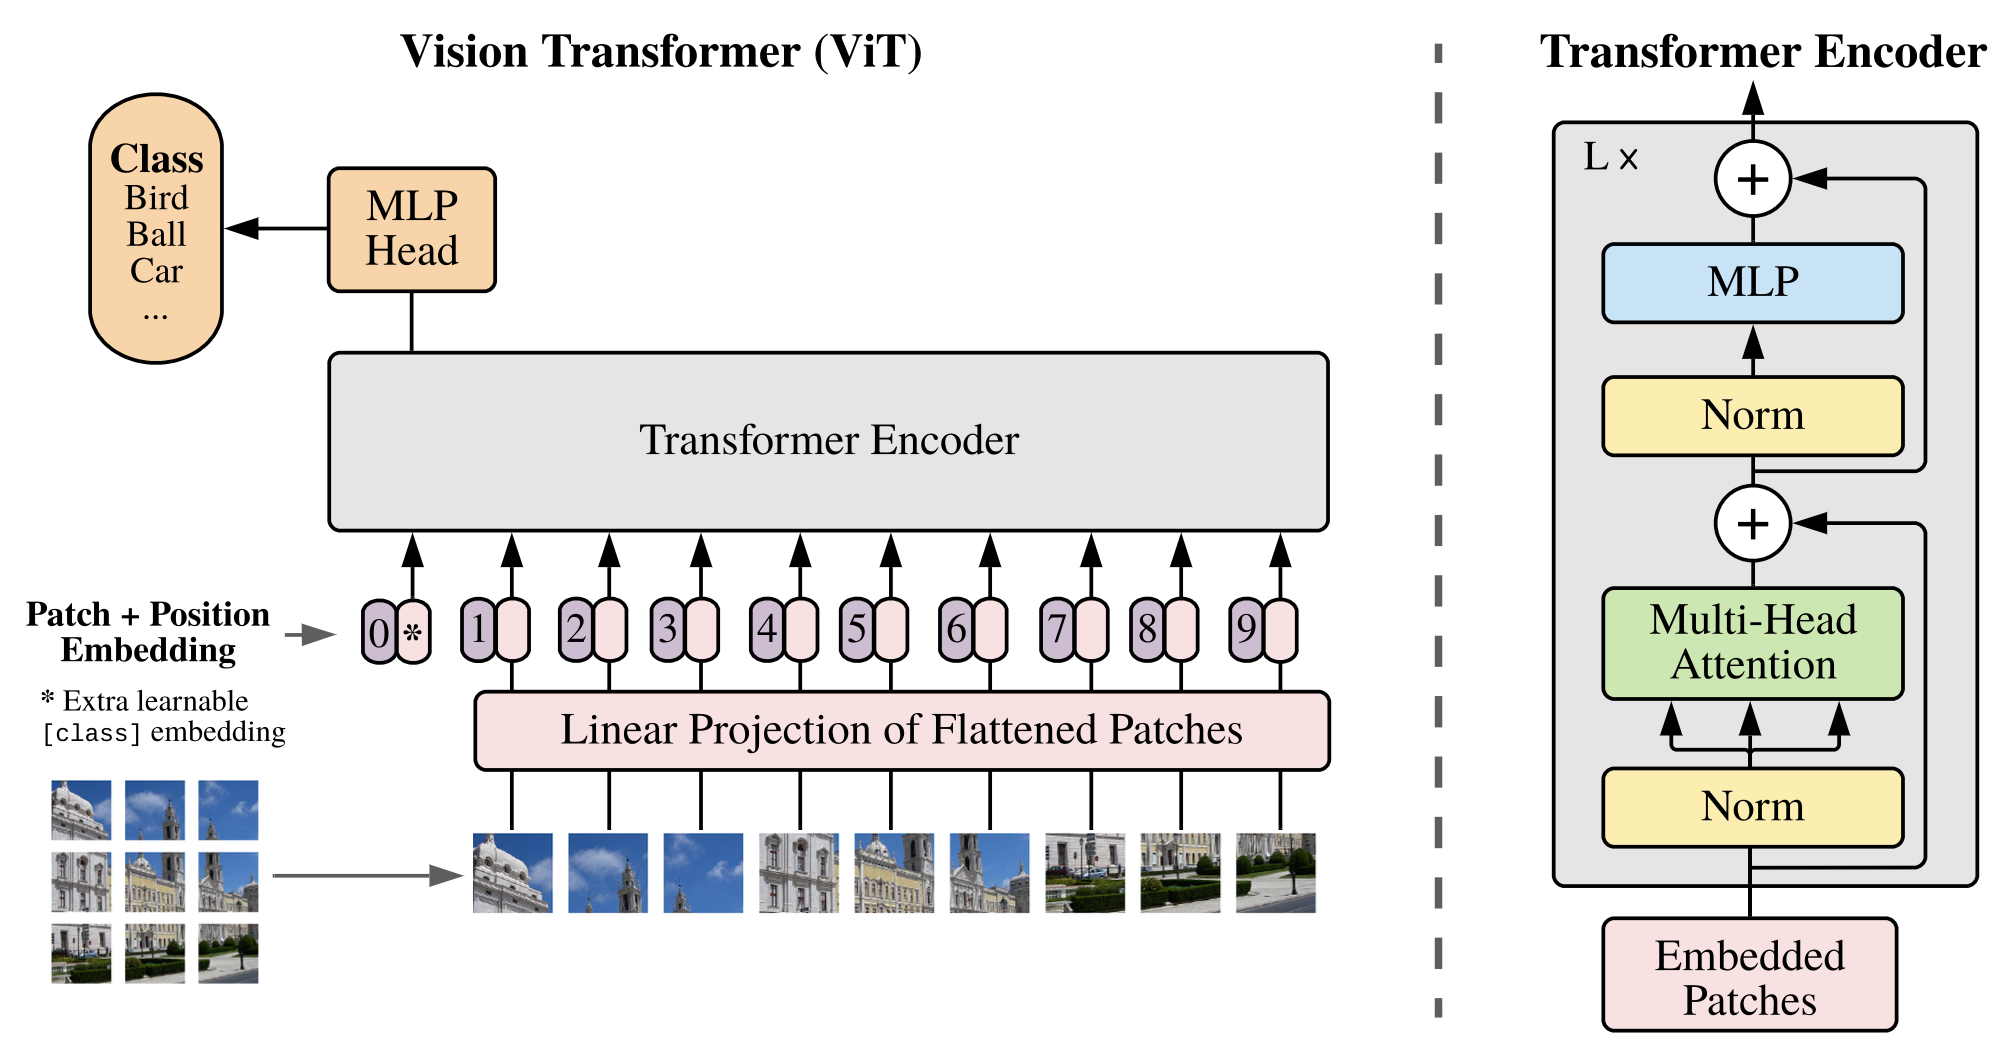
\includegraphics[width=\linewidth]{assets/vit_overview.png}
    \caption{\label{fig:vit_overview}The overall architecture of ViT.}
\end{figure}


{\small
\bibliographystyle{ieee}
\bibliography{egbib}
}

\end{document}
